\chapter{Methodology}
% (diagram: data flow ; from input to output, everything in between; a paragraph on each module)

\section{Machine Learning Workflow}
The Machine Learning workflow used in this Master thesis is based upon a universal blueprint proposed by \citet{Chollet:2017:DeepLearningPython}. The blueprint consists of the following seven steps, outlined below, followed by a few keywords describing the approach proposed by this Master's thesis.

\begin{enumerate}
    \item \textbf{Defining the problem and assembling a dataset}\newline
    Emotion Recognition, Regression problem, AFEW-VA dataset
    \item \textbf{Choosing a measure of success}\newline
    RMSE, CORR
    \item \textbf{Deciding on an evaluation protocol}\newline
    5-fold-Cross-Validation
    \item \textbf{Preparing your data}\newline
    Restructure frames, resize the range of label's value
    \item \textbf{Developing a model that does better than baseline}\newline
    Implementing a first model that performs better than by chance
    \item \textbf{Scaling up: developing a model that overfits}\newline
    Implementing the pre-trained neural network ResNet50
    \item \textbf{Regularizing your model and tuning your hyperparameters}\newline
    Dropout, DataAugmentation
\end{enumerate}



\section{Research paradigm: Ablation Study}

\begin{quote}
    An Ablation Study, in medical and psychological research, is a research method in which the roles and functions of an organ, tissue, or any part of a living organism, is examined through its surgical removal and observing the behaviour of the organism in its absence.\citep[~p. 15]{Sheikholeslami:2019:AblationProgrammingML}
\end{quote}


Ablation Study, in the context of Machine Learning, is derived from its medical/psychological background. \citet{Sheikholeslami:2019:AblationProgrammingML} described Ablation study as a scientific examination of a \gls{ML} system by purposefully removing features or components in order to observe its effects on the system's performance wherein every design choice or module can be included. Ablation Study, therefore, allows for the gleaning of valuable insights; however it doesn't have the capability to provide sufficient proof to draw direct conclusions regarding the module's contribution.
\newline\newline
The idea behind Ablation Study being applied to Artificial Neural Networks (ANNs) in this Master's thesis was to make a Neural Network perform better on Emotion Recognition than its baseline. After this step was completed, modules or design choices were removed from the network in order to analysis outcomes separately. According to \citet{Fadelli:2018:AblationInANN}, this allows the researcher to measure the performance change due to the caused damage.


% \subsection{Development technique: Minimum Viable Product (MVP)}
% The concept of a Minimum Viable Product (MVP) was first introduced by \citet{Ries:2011:TheLeanStartUp} as a methodology for creating a 'Lean StartUp'. It aims at starting the learning process as early as possible through integrating early adopter's feedback.\citep{Lenarduzzi:2016:MVP}
% \newline\newline
% \citet{Lenarduzzi:2016:MVP} argues that the Build-Measure-Learn loop is one of the core principles in 'Lean StartUp' which allows entrepreneurs to learn whether to give up or persevere with a current build. This build is usually defined as a MVP. The author \citet{Ries:2011:TheLeanStartUp} describes an Minimum Viable Product as follows:
% \begin{quote}
%     "The MVP is that version of the product that enables a full turn of the Build-Measure-Learn loop with a minimum amount of effort and the least amount of development time." \citep{Ries:2011:TheLeanStartUp}
% \end{quote}
% However, \citet{Ries:2011:TheLeanStartUp} clarifies that a MVP is still far from being complete, on the contrary, it requires additional effort during building as its outcomes will be presented to potential customers and its feedback needs to be measurable. 
% \newline\newline
% The MVP for this this starts off with just the code for training a artificial neural network and testing its achievements on previously unseen data. This allowed the author to show a fully functioning product from the beginning on and to add functionality with the progress of the experiments.
% \newline\newline
% While the MVP is being expanded the measurable results are being presented continually to the supervisors from the University of Hamburg, as well as the supervisor from PPI AG. The resulting feedback flows back into the product by the design of the future experiments and changes. Thus, following the philosophy of the MVP, allowed the author to steer the direction of the experiments as needed and to continually receive actionable feedback on the current state of the product.

    
%%%%%%%%%%%%%%%%%%%%%%%%%%%%%%%%%%%%%%%%%%%%%%%%%%%%%


\section{Methods}	

The approach proposed in this Master's thesis was composed of multiple methods \ref{fig:MachineLearningModelMethods}. The left hand side of the figure is a summary of the approach, in consecutive order, from top to bottom. Each step has a number assigned to it, which can be found on the right hand side with a corresponding example picture of the output of the said step.

\begin{figure}[H]
  \begin{center}
  \makebox[\textwidth][c]{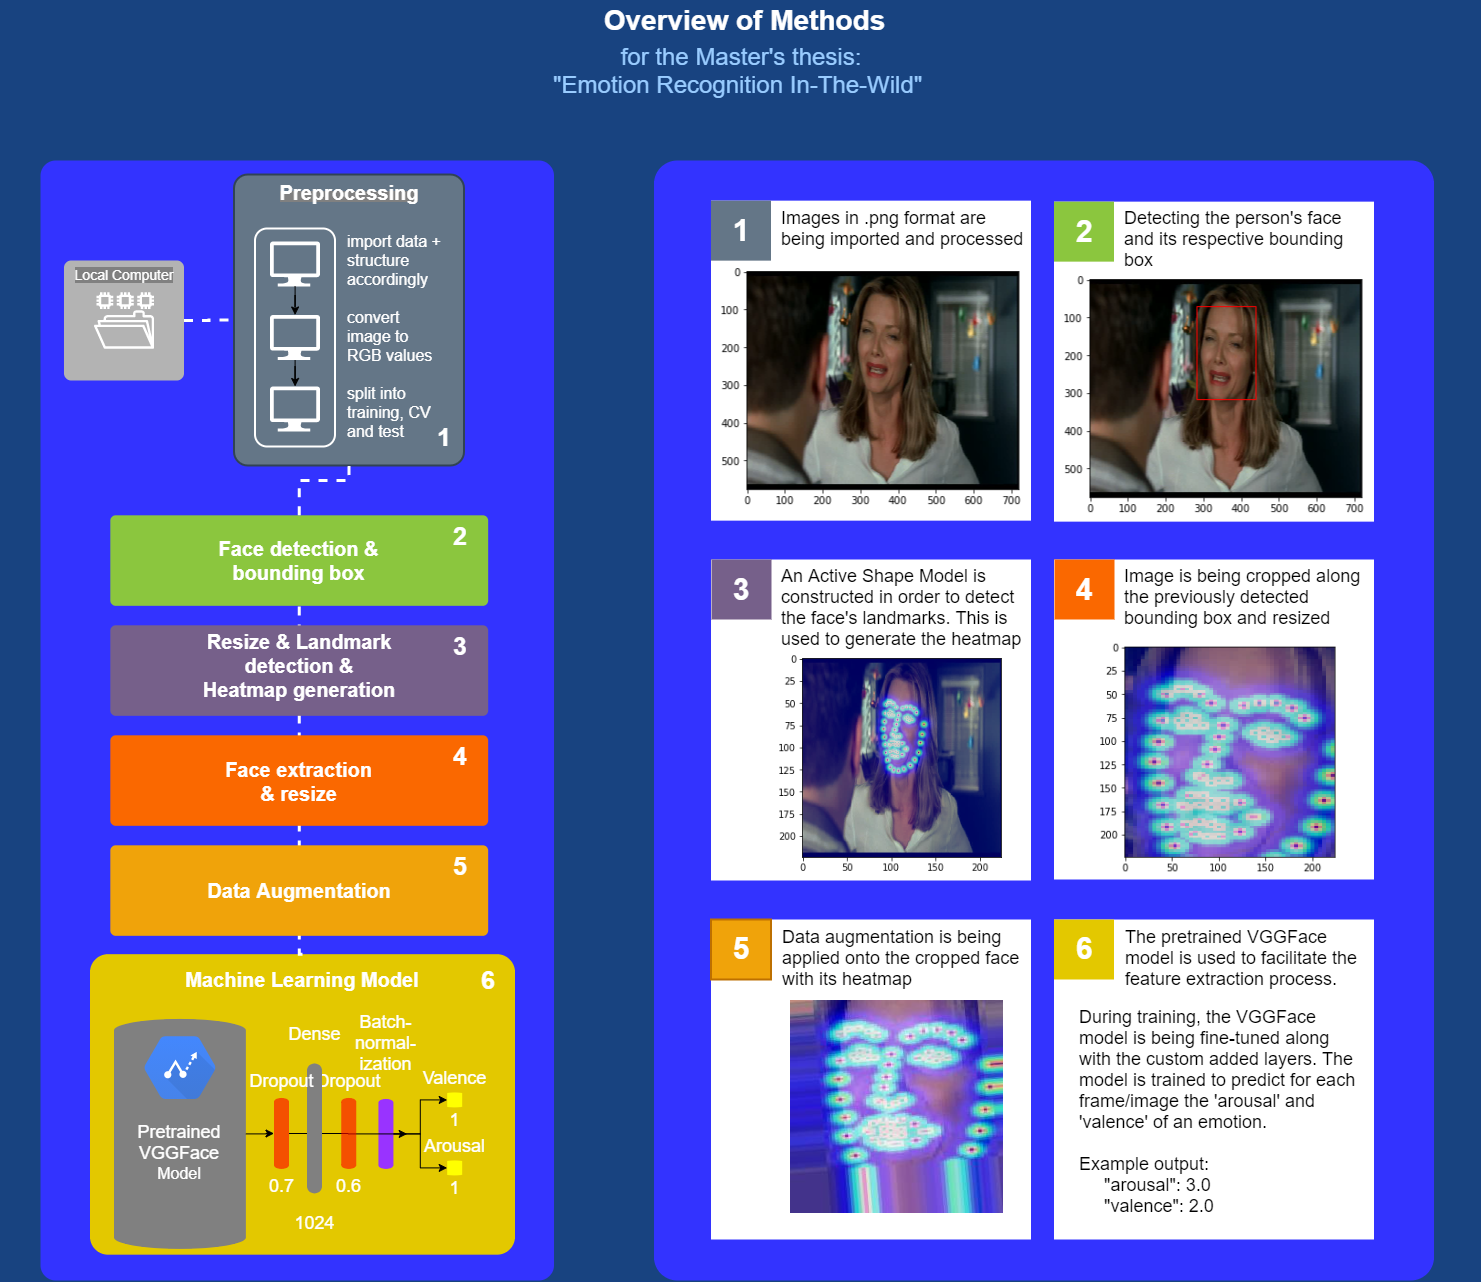
\includegraphics[width=1.2\textwidth]{Figures/DataFlow_Diagram.png}}%
  %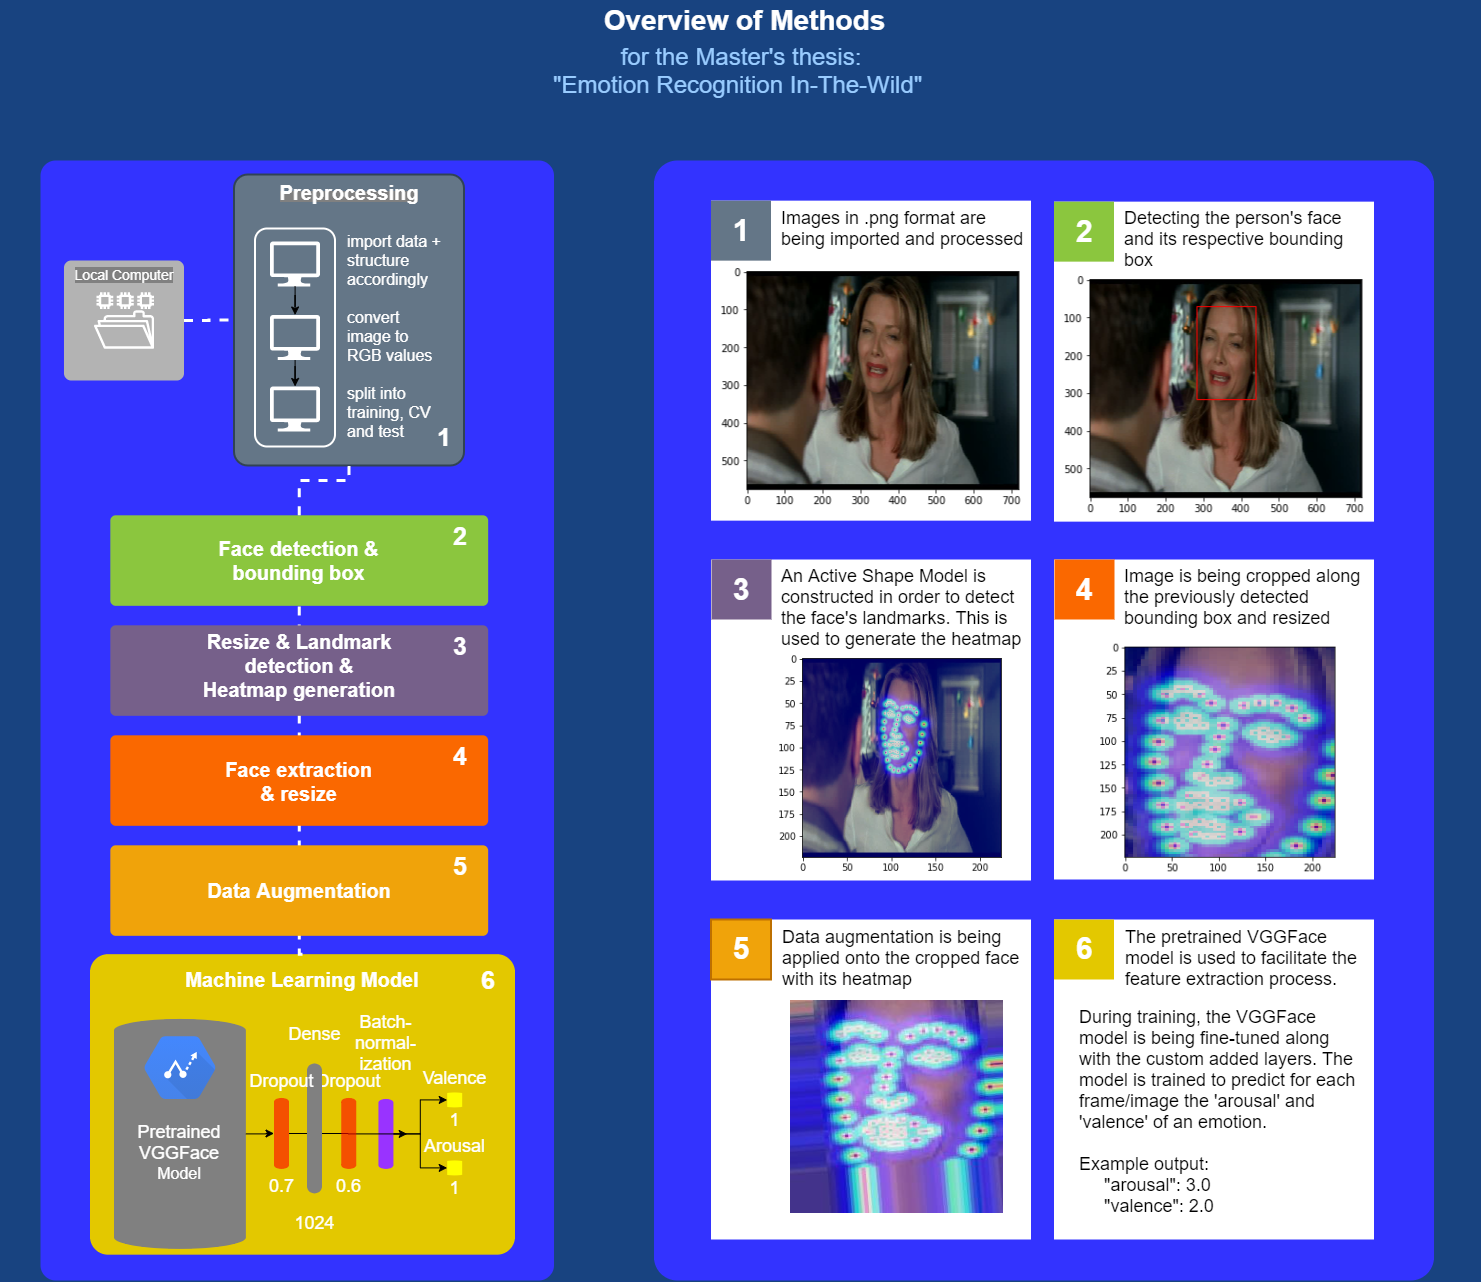
\includegraphics[angle=0, width=1.0\textwidth]{Figures/DataFlow_Diagram.png}
  \caption{Overview: Machine Learning Model - Methods}
  \label{fig:MachineLearningModelMethods}
  \end{center}
\end{figure}


\subsection{Preprocessing}
Before any approach could be implemented that automatically read in frames of video clips and their respective target labels in a specific data structure, the data structure of the selected database had to be analyzed.
\newline\newline
Afterwards, a program was written, that automatically created a list of filenames for all the (video-)frames inside the database, along with corresponding labels for valence and arousal. Based on the list of file names, actual image data was read in and converted into RGB values. Data got split into five different folds, each containing about 20 \% of subject-independent video clips, in order to facilitate a separation of data into training, validation and testing data at a later stage.
\newline\newline
Furthermore, the target values of valence and arousal were brought into the same data structure. Additionally, the values were divided by a factor of 10, as the labels had to be brought into a range of -1 to 1 in order to fit the 'tanh' activation function of the model's final output layer. The following figure is a plot representing the outcome of the preprocessing step together with its target values.
% While the training data set is being shuffled for a better generalization during training, the testing data is used for validating the training results on a previously unseen part of the dataset.

% The last preprocessing step involves loading all the images, converting it into RGB values and then extracting the face while using the face detection techniques described in the next chapter. The cropped output image will have a shape of 224x224x3 and will be permanently saved so that this step doesn't have to be repeated each time the model is being trained. Furthermore, the model can then reach back to this array of extracted images and directly use them to train or finetune the model.

\begin{center}
\begin{figure}[H]
  \begin{center}
  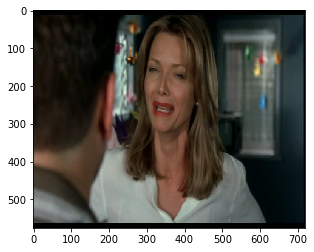
\includegraphics[angle=0, width=0.5\textwidth]{Figures/method_1.png}
  \caption{Method 1}
  \label{fig:MachineLearningModelMethod_1}
  \end{center}
\end{figure}
\end{center}

\begin{table}[H]
\begin{center}
\begin{tabular}{@{}ccc@{}}
\toprule
 & Valence & Arousal \\ \midrule
\multicolumn{1}{r}{label / target} & - 0.5 & + 0.3 \\ \bottomrule
\end{tabular}
\caption{Label / Target of input image}
\label{tab:LabelTarget}
\end{center}
\end{table}


\subsection{Face Detection \& Bounding Box}
The \gls{MTCNN} proposed by \citet{Zhang:2016:MTCCN} is a pre-trained neural network optimized for the tasks of simultaneous face detection, face alignment, bounding boxing and landmark detection \citep{Brownlee:2019:VggFace2HowToFaceRec}.
\newline\newline
In this Master's thesis, the \gls{MTCNN} model was used to detect the face in an image and determine its coordinates for the bounding box. Thus, after successful performance of the preprocessing step, the \gls{MTCNN} module detected the face and determined its bounding box. For illustration purposes, a rectangle was drawn on the following figure, corresponding to the bounding box coordinates determined by the \gls{MTCNN} module.

\begin{center}
\begin{figure}[H]
  \begin{center}
  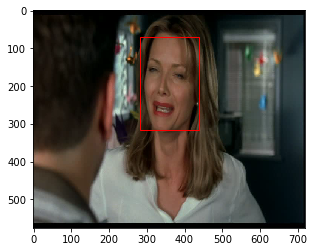
\includegraphics[angle=0, width=0.5\textwidth]{Figures/method_2.png}
  \caption{Method 2}
  \label{fig:MachineLearningModelMethod_2}
  \end{center}
\end{figure}
\end{center}

\subsection{Landmark detection \& Heatmap generation}
The pre-trained 'Face Landmark Detection' algorithm \citep{Kazemi:2014:ShapePredictor} from the dlib library was implemented in order to detect 68 facial landmarks of a person's face. This algorithm determined landmarks by creating a shape model that is successively aligned to the specific features of the face at hand with the help of a cascade of regressors.
\newline\newline
For the implementation, the shape predictor requires, next to the input image, the bounding box of the person's face appearing in the input image. As the bounding box was already determined during the previous step by the \gls{MTCNN} module it was being used as an input for the landmark detection. \citep{Datahacker:2020:DlibFacialLandmarks}
\newline\newline

\begin{quote}
    imgaug is a library for image augmentation in machine learning experiments. It supports a wide range of augmentation techniques ... it can not only augment images, but also keypoints/landmarks, bounding boxes, heatmaps and segmentation maps. \citep[~para. 1]{Jung:2020:Imgaug}
\end{quote}
Imgaug was used to convert the previously detected landmarks into a heatmap and to apply it as an overlay onto the image.

\begin{center}
\begin{figure}[H]
  \begin{center}
  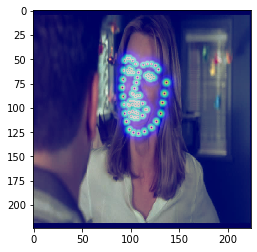
\includegraphics[angle=0, width=0.5\textwidth]{Figures/method_3.png}
  \caption{Method 3}
  \label{fig:MachineLearningModelMethod_3}
  \end{center}
\end{figure}
\end{center}

\subsection{Face Extraction}
The input for this step consisted of the image with a heatmap as an overlay, as well as the coordinates for the face's bounding box. Hence, the face was simply cropped along the lines of the rectangle, composed of the bounding box's coordinates. % \citep{Brownlee:2019:VggFace2HowToFaceRec}

\begin{center}
\begin{figure}[H]
  \begin{center}
  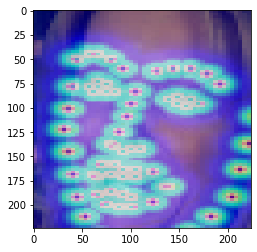
\includegraphics[angle=0, width=0.5\textwidth]{Figures/method_4.png}
  \caption{Method 4}
  \label{fig:MachineLearningModelMethod_4}
  \end{center}
\end{figure}
\end{center}

A new image was created with the heatmap integrated into the RGB image. Thehe shape dimension of the image stayed the same, as required by the pre-trained Neural Network. However, the image was first utilized for data augmentation purposes.

\subsection{Data Preparation}
After the face was extracted from all the frames, the data had to be prepared in order to be finally consumed by the Neural Network.
\newline\newline
Firstly, data standardization was conducted which had to be the same as the one used for VGGFace model pre-training. The authors of the keras-vggface library provided a method that does this standardization method by subtracting the training mean for all three image channels. This function was applied in this thesis which resulted in the mean for each channel being equal to zero.
\newline\newline
Afterwards, the data was split into training, validation and testing in a subject-independent manner. The training data was fed into the Data Augmentation model, the validation went directly as input into the model's training process, and testing data was utilized during the evaluation of the model.

\subsection{Data Augmentation}
In order to improve the model's generalization capabilities, Data Augmentation was applied beforehand to the training images using the ImageDataGenerator provided by Keras. It worked as follows:
\begin{itemize}
    \item Taking a batch of training images
    \item Apply random transformations on it
    \item Replace the original batch with the newly transformed batch
\end{itemize}
Data was transformed randomly in terms of rotation, width shift, height shift, horizontal flip, brightness and zoom.

\begin{center}
\begin{figure}[H]
  \begin{center}
  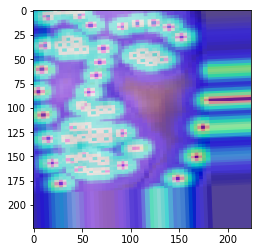
\includegraphics[angle=0, width=0.5\textwidth]{Figures/method_5.png}
  \caption{Method 5}
  \label{fig:MachineLearningModelMethod_5}
  \end{center}
\end{figure}
\end{center}


\subsection{Machine Learning Model for Emotion Recognition}
As Emotion Recognition poses similar challenges for researchers as Face Detection, the goal was to reuse already learnt abstractions and facial features from the pre-trained VGGFace Neural Network optimized for face detection challenges. This Neural Network model was then further fine-tuned on the AFEW-VA dataset during this research which should lay the foundation for high quality results at the Emotion Recognition at hand.
\newline\newline
The VGGFace model architecture is based on the famous ResNet-50 Convolutional Neural Network which the authors \citet{Cao:2018:VGGFace2} pre-trained on a large-scale face dataset, named VGGFace2. The dataset contains about 3.31 million images of 9131 subjects and poses, which provided a wide variety of poses, ages, etc. When the VGGFace2 paper written by \citet{Cao:2018:VGGFace2} was published in \citeyear{Cao:2018:VGGFace2}, its performance exceeded the previous state-of-the-art by a large margin \citep{Cao:2018:VGGFace2}.
\newline\newline
Due to the fact that VGGFace is optimized for face recognition, it had to learn similar facial features to what was required by Emotion Recognition. Therefore, the weights of the VGGFace model already encapsulate the extracted information from a person's facial features. However, the classifier of the model, usually consisting of a few Dense layers at the end of the mode, was not reusable. Instead it got trimmed in order to allow the newly added classifier to learn the correlation between facial features and the target labels of the Emotion Recognition challenge. As a result, the last Dense layers was replaced by custom made layers consisting of a Dropout layer, a single Dense layer with 1024 units, another Dropout layer, a Batch Normalization layer and two Dense layers, one for each output value.